\subsection{深入调研——冷启动问题}
在之前的文献综述过程中,我们较为详细地讨论了推荐系统的发展过程,以及实现的方法与模型。但是对于推荐问题,仍然有一些潜在的问题,可能会较大地影响推荐系统的结果\cite{currentprob}。其中一大问题就是冷启动问题。冷启动问题在音乐推荐系统中表现地尤为明显,由于音乐的数量很大,用户对于音乐的评分矩阵往往是稀疏的。所以音乐推荐系统中,冷启动的影响是较大的。所以我们首先对于这一问题的解决方法进行了更深入的探究。

\subsubsection{冷启动问题的分类}
在现有的研究中,研究者将冷启动问题进行细分,分成了两部分问题。一类是CCS,表示用户或者音乐完全是新的,没有历史的交互数据,这就导致了部分的模型是完全不工作的。另一类是ICS,表示用户或音乐是有一部分交互信息的,但是这部分的交互信息对于描述用户评分特征上来看是不够充分的,此时给出的推荐结果也是不可靠的,可能会影响到用户的使用体验。

\subsubsection{冷启动问题的相关工作}
对于推荐系统中的冷启动问题,已经有了一部分相关的工作,来解决这一问题。具体的解决方法有如下几种\cite{currentprob}:
\begin{itemize}
    \item Content-Based方法
    \item 混合模型
    \item Cross-Domain模型
    \item Active Learning
\end{itemize}

这四种方法的主要思路大体是相似的,都是利用用户和音乐的其他信息来对于交互项进行补充,从而加强对于用户和音乐特征的建模。

此外,从推荐系统之外的领域,也有一些关于缺失数据的处理过程可供借鉴。比如图片分类问题,一些完全没有见过的图片,我们需要对其进行分类的问题为Zero-Shot的问题,而对于一些出现次数较少的图片,其分类问题为Few-Shot问题。这两种问题中,Zero-Shot问题可以和推荐问题中的CCS问题对应,而Few-Shot问题可以与推荐问题中的ICS问题对应。所以我们可以参考图片分类问题中对于Few-Shot问题和Zero-Shot问题的处理,给出相似的解决方案\cite{currentprob}。

\begin{figure}[htb]        
\center{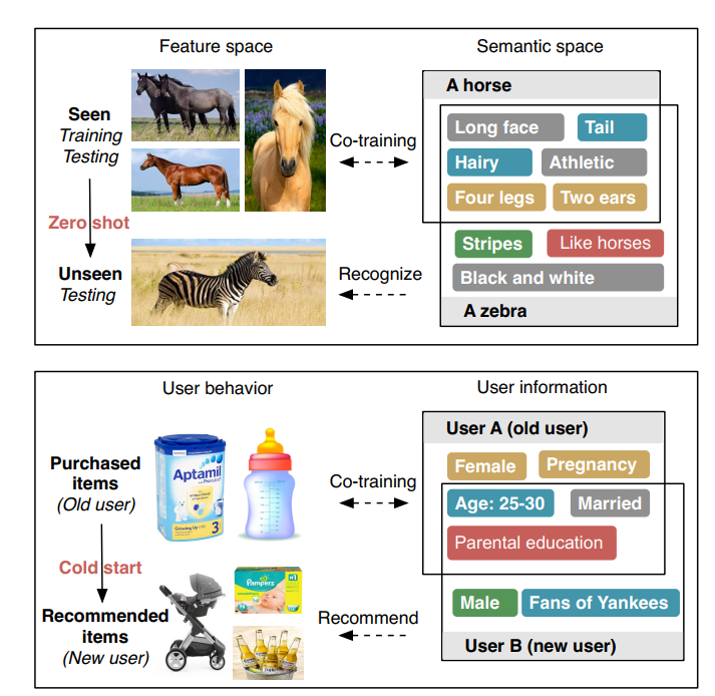
\includegraphics[width=10cm]  {MusicRecomSurvey/pics/zero-shot.png}}    
\caption{\label{1} Zero-Shot方法}      
\end{figure}

\begin{figure}[htb]        
\center{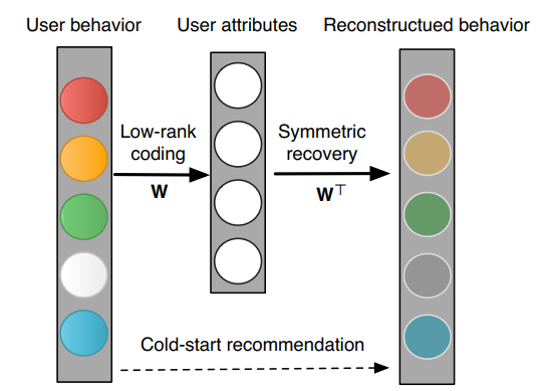
\includegraphics[width=8cm]  {MusicRecomSurvey/pics/autoencoder.png}}    
\caption{\label{2} AutoEncoder方法}      
\end{figure}
一种方法是使用用户信息及物品信息,如图1所示,如果我们能够采集有效的信息,就可以在此基础上进行一定的推断,得出用户对于一些物品的喜爱程度。在此基础上,可以更进一步,使用AutoEncoder的结构,对于特征进行提取,如图2所示。此时对于冷启动的用户,通过AutoEncoder先进行编码,再进行解码,则最后解码得到的值就包含了该用户在这里通过用户特征推测出的值\cite{zeroshot}。

另一种方法将这一问题转化为了Meta-Learning的问题,使用Meta-Learning的方法来解决冷启动的问题\cite{metalearning}。如图3所示。
\begin{figure}[htb]        
\center{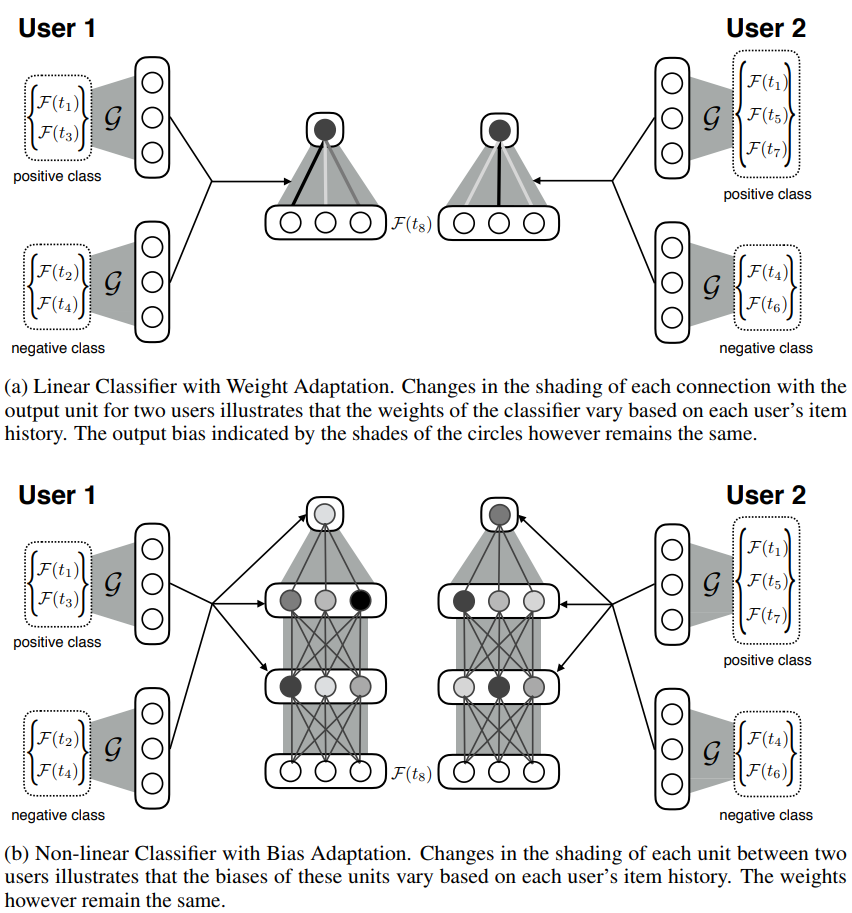
\includegraphics[width=8cm]  {MusicRecomSurvey/pics/meta.PNG}}    
\caption{\label{3} Meta-Learing方法}      
\end{figure}

\subsubsection{我们的研究思路}
在调研过程中,我们发现对于冷启动问题,CCS和ICS两个子问题在解决方法上也存在一定的差异\cite{coldstart},所以我们认为不一定要设计出一个模型,来对两个子问题都找到较好的解法。所以我们在设计自己的模型时更加注重于对于ICS问题。希望能尽可能高效地利用有限的评分信息,对于用户的评分习惯进行更准确的分析。

同时,借鉴了CV领域中的Relation-Learning的思想,我们希望能够使得推荐系统能够通过一种更加准确的方式来学会如何“比较相似性”。在此基础上,我们调研了在推荐系统中运用Metric-Learning的情况,发现虽然这些方法已经初步有了使推荐系统学习距离信息来推测相似度的相关想法,但是其优化的距离或者说用于定义相似度的距离都是低阶线性的距离算法。这种方法虽然可以给出一定的距离描述,但是难以对于神经网络提取的高阶特征进行充分的捕捉和利用。所以我们希望能够通过Relation-Learning中计算图片与图片之间相似度的方法,应用到推荐系统中用于计算人与人,音乐与音乐,用户与音乐之间交互等的相似性。

所以我们的模型的基本思路就确定为一个混合推荐模型,使用Relation-Learning的思路,学习用户评分的相似性,之后通过协同过滤,对于评分的值进行估计。